Fill in the table on page 2.
%\begin{figure}[ht]
%    \centering
%    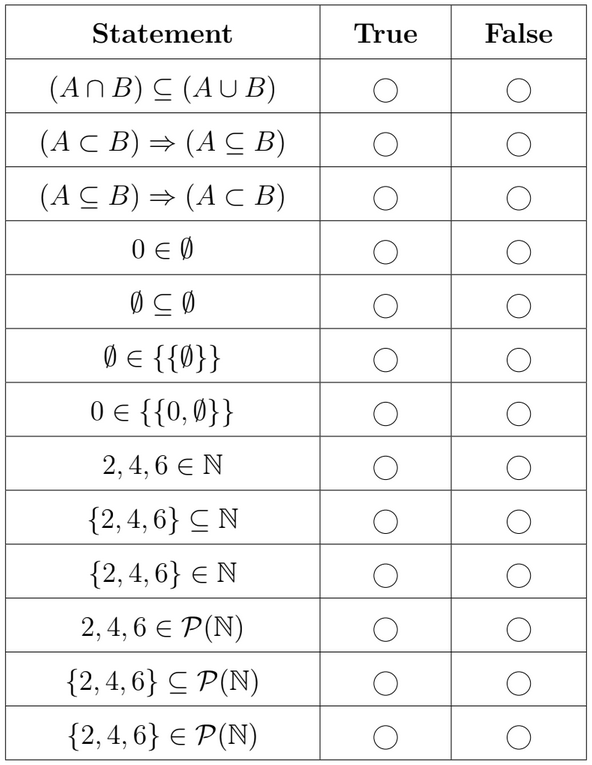
\includegraphics{Ch3/004.PNG}
%    \label{fig:tf}
%\end{figure}

Here are some definitions we will go over. $A$ and $B$ denote any sets.
\begin{itemize}
    \item $x \in A$ means an object $x$ is in the set $A$.
    \item $A \cup B = \{x \mid (x \in A) \lor (x \in B)\}$.
    \item $A \cap B = \{x \mid (x \in A) \land (x \in B)\}$.
    \item $A \subseteq B \iff ((x \in A) \implies (x \in B))$.
    \item $A \subset B \iff (A \neq B) \land (A \subseteq B)$.
    \item $\mathcal{P}(A) = \{U \mid U \subseteq A\}$. This is the \textbf{powerset} of $A$. 
    \item $|A|$ simply denotes the number of elements in the set $A$. For example, $|\{1, 2, 3\}| = 3$.
\end{itemize}